% !TEX root = ../main.tex
\section{Introduction}
\label{introduction}

An often cited statistic is that data scientists spend 80\% of their time finding, preparing, integrating and cleaning data sets. The remaining 20\% time is spent doing the desired analytic tasks such as data mining and machine learning. In fact, 80\% may be a lower bound; for example one data officer, Mark Schreiber of Merck, a large pharmaceutical company, estimates that data scientists in Merck spend 98\% of their time on the ``grunt work'' and only one hour per week on ``useful work''.

In this paper, we present \dcv, a system we are building at MIT, QCRI, Waterloo, and TU Berlin, whose main purpose is to decrease the ``grunt work factor'' by helping data scientists in 
(i)~performing data discovery, i.e., quickly find data of interest from large numbers of tables;
(ii)~computing a linkage graph, i.e., find ways to connect data sets of interest;
(iii)~executing queries to fetch desired data from disparate data stores;
(iv)~cleaning the required data; and %as it is often cited that 20\% of a typical data source is incorrect or missing; and
(v)~performing these tasks iteratively using a workflow system since data scientists often iterate through these steps in different orders.

%\vspace{.5em} %Mourad: It's ugly with this space thing!
%\begin{itemize} \\

%
%\begin{enumerate}[label=\roman*)]
%
%%\noindent i)
%\item perform data discovery; i.e., quickly find data of interest from large numbers of tables,
%
%%\vspace{.5em}
%%\noindent ii)
%
%\item perform data stitching; i.e., find ways to connect data sets of interest,
%%\vspace{.5em}
%
%%\noindent iii)
%\item execute queries to fetch desired data from disparate data stores,
%
%%\vspace{.5em}
%
%%\noindent iv)
%\item clean the required data, as it is often cited that 20\% of a typical data source is incorrect or missing,
%
%%\vspace{.5em}
%
%%\noindent v)
%\item perform these tasks iteratively using a workflow system since data scientists often iterate through these steps in different orders.
%
%%\vspace{.5em}
%\end{enumerate}

\dcv consists of a collection of modules with a workflow scheduling system, as noted in the architecture diagram of 
Figure~\ref{fig:arch}. We elaborate on each module in the remainder of this section, using Merck as an example.
We should note that \dcv focuses on structured data, which are represented as a collection of (sparse or dense) tables.


\begin{figure}[!t]
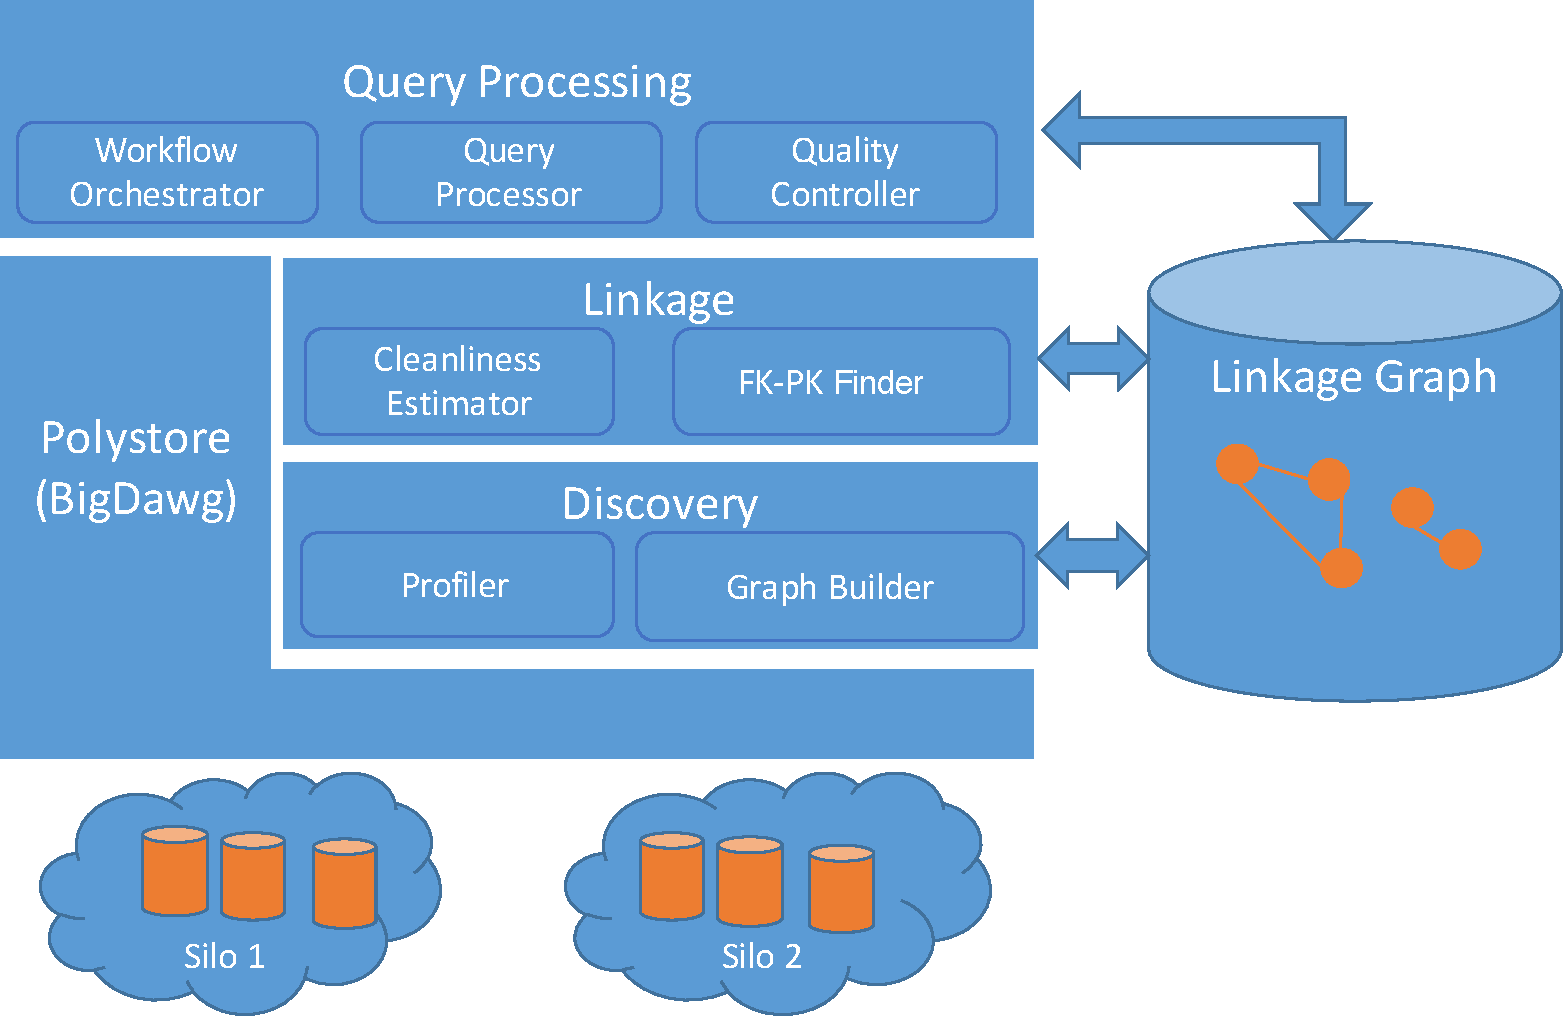
\includegraphics[width=3.5in]{arch3.pdf}
\caption{\dcv Architecture}
\label{fig:arch}
\end{figure}


\stitle{[Discovery.]} 
A data scientist at Merck has a hypothesis, for example, {\it the drug Ritalin causes brain cancer in rats weighing more than 300 grams}.
His first job is to identify relevant data sets, both inside and outside of Merck, that might contribute to testing this hypothesis. Inside the company alone, Merck has approximately 4,000 Oracle databases and countless other repositories. The discovery component in \dcv, will assist the scientist in finding $m$ tables of interest from all $n$ tables such that $m \ll n$, where $n$ is the number of all tables making it much bigger than 4000.  
%
The process of discovering relevant tables is typically in the granularity of columns. 
%Assume that each table has a constant number of columns in average, which is usually true in practice. 
Thus, only linear algorithms, i.e., those that can run in $O(n)$ time, are computationally feasible.
%Assuming that each table has up to $c$ columns, only linear algorithms, i.e., those run in $O(c\cdot n)$ time, are computationally feasible. If we also assume w.l.o.g. that $c$ is a constant, the discovery has to run in $O(n)$ time.
%
This module, together with the corresponding data structures, will be discussed in Section~\ref{sec:discovery}.

%Since discovery must be run on millions of columns, we assume that only linear algorithms are computationally feasible, and any needed data structures must be built in advance.

\stitle{[Linkage Graph Computation.]} 
The semantic linkage between attributes of discovered tables is extremely helpful in constructing a composite \textsf{SQL} query to access the discovered data sets. 
%
Our current prototype leverages primary key-foreign key relationships (inclusion dependencies) for this purpose.
Assuming a constant number of attributes in each table, there may exist up to $O(m^2)$ linkages among different attributes.
%It may have up to $O(m^2)$ linkage among different attributes, assuming a constant number of columns each table holds in average.
%
%Given $n$ data sets and each has up to $c$ attributes, in the worst case there are $O(n^2)$ linkages among different attributes, by treating $c$ as a constant.
Since $m$ is typically small, being the result of data discovery,\mourad{Should we mention here that we may need more tables beyond the discovery module's output to build join paths? It might be confusing as this stage.}
the process of building the linkage graph can be run dynamically; we discuss its details in Section~\ref{sec:stitching}.

%The discovery and stitching modules share a common graph structure. Such structure has a node for each column in each table with various kinds of links such as data similarity, schema similarity, and inclusion dependency.  These links are maintained in a data fabric similar in spirit to a knowledge graph~\cite{DBLP:conf/semweb/AuerBKLCI07,DBLP:conf/sigmod/BollackerEPST08,DBLP:conf/www/SuchanekKW07}. Building and maintaining this graph is the responsibility of the graph builder component.


\stitle{[Polystore Query Processing and Curation.]}
Since organizations such as  Merck have a variety of massive-scale data storage systems, it is not feasible to move all data to a central data warehouse. Also, it is neither economically nor technically practical to perform data processing on all of the thousands of databases in advance. 
\dcv is built using a polystore architecture~\cite{DBLP:journals/sigmod/DugganESBHKMMMZ15}, where all modules assume a polystore computing environment.
Using the \texttt{BigDAWG} polystore system~\cite{DBLP:journals/pvldb/ElmoreDSBCGHHKK15}, we can pull data out of multiple underlying storage engines as needed to compute the final result (or a {\em view}) to meet the user specification, i.e., his/her hypothesis. 

%\stitle{[Curation Polystore]} 

%In fact, we are building on the \texttt{BigDAWG} polystore system~\cite{DBLP:journals/pvldb/ElmoreDSBCGHHKK15}. The polystore architecture can pull data out of multiple underlying storage engines as needed. 

Obviously, data cleaning, data transformation and entity consolidation must be integrated with querying the polystore and constructing the desired user view.  
This is an expensive process with the human effort required to validate cleaning decisions being the most important cost. 
Since there may be multiple views that ``solve'' a data scientist's query, each with different accuracy and human validation cost, \dcv must estimate the cost of curating the possible views,
%to reason about the feasibility of using each one,
given a scientist's time budget. 


%Obviously, we want to run stitching in the background in advance to deliver the best possible response time. As noted in Section~\ref{sec:stitching}, our current prototype leverages PK-FK relationships (inclusion dependencies).
%We also plan to explore other possible relationships in the futu%The merger of polystores and data curation steps is discussed in Section~\ref{sec:curating}.re such as ???.
%Effectively, the result of stitching is a ``view'' of multiple data sources that contains the composite data of interest to the scientist.


%\stitle{[Cleanliness Estimation]} 
%Indeed, \dcv is an iterative process, the human effort will be involved in various modules. The expensive process in constructing the view mentioned above is the human effort required to validate cleaning decisions. Since there may be multiple views that ``solve'' a data scientist's query, each with different accuracy and human validation cost, \dcv must estimate the cost of curating the possible views,
%%to reason about the feasibility of using each one,
%given a scientist's time budget. 

The above aspects will be discussed in Section~\ref{sec:curating}.
%Estimating the cleanliness of a view entails constructing a model for the dirtiness of the data in each source data set, which we discuss in Section~\ref{sec:curating}. Also discussed in Section~\ref{sec:curating} is where in a query plan we should allocate a cleaning budget.


%\stitle{[Optimizing Stitching]} It is highly inefficient and wasteful to  discard expensive-to-construct materialized views after their initial use by a data scientist.  Hence, we assume that they are generally retained for future use.  Moreover, future materialized views  may be based off previously constructed ones or on original data sources.  As a result, there may be several ways to construct a new view, with different  costs and accuracy. Therefore, the data stitching problem must be revisited to deal with this materialization cost/accuracy trade-off.  This is the subject of Sections~\ref{sec:enhancedstitching}.\mourad{Why not merge this section with Data Stitching?}

\stitle{[Updates.]}  
If a source data set is updated, these updates must be incrementally propagated through the data curation pipeline to update downstream materialized views. 
In some cases, the human effort involved may be daunting and the materialized view should be discarded rather than updated. 
In addition, if a scientist updates a view, we need to propagate changes to other derived views, as well as back upstream to data sources, if this is possible. Section~\ref{sec:updates} discusses these  issues.



\stitle{[Workflow.]} 
\dcv offers a workflow engine whereby data scientists can iterate over its components in whatever order they wish,  Moreover, they need to be able to undo previous workflow steps and perform alternate branching from the result of a workflow step.  Section~\ref{sec:workflow} discusses our workflow management.

\smallskip

We describe the current implementation of \dcv in Section~\ref{sec:wild}. We also report on initial user experience for two use cases: the MIT data warehouse and Merck. We conclude with final remarks and an outline of our future research plans in Section~\ref{sec:conclusion}.


\stitle{Our contributions.}
The main contribution of \dcv is that it is an ``end-to-end'' system. In contrast, there has been much work on ``point solutions'' that solve small pieces of the overall problem. For example, Data Wrangler~\cite{2011-wrangler} and DataXFormer~\cite{DBLP:conf/icde/AbedjanMIOPS16} automate some aspects of cleaning and transforming data.
In addition, we studied several representative data cleaning systems on a collection of real world data sources ``from the wild''~\cite{DBLP:journals/pvldb/AbedjanCDFIOPST16} and we found out that there was no cleaning Esperanto and multiple tools are required to achieve reasonable accuracy.  
Hence, point solutions do not achieve acceptable performance, and an ensemble approach is required.
%
Data Tamer~\cite{DBLP:conf/cidr/StonebrakerBIBCZPX13} performs schema mappings and record linkage. DeepDive~\cite{DBLP:journals/pvldb/ShinWWSZR15} extracts facts and structured information from large corpora of text, images and other unstructured sources. However, neither solution performs  discovery, linkage graph computation, and polystore operations in concert.

